\begin{align}
\because \vec{A}-\vec{B} 
&=\myvec{1\\-3}-\myvec{-2\\1} \\
&=\myvec{3\\-4}, 
\label{1/8/eq5}
\end{align}
Hence, 
\begin{align}
\norm{\vec{A}-\vec{B}}&= \sqrt{\myvec{\vec{A}-\vec{B}}^\top\myvec{\vec{A}-\vec{B}}}\\
&=\sqrt{\myvec{3& -4} \myvec{3\\-4}} \\
&=\sqrt{3^2 + \myvec{-4}^2} \\
&=5 
\end{align}
\begin{figure}[!ht]
	\centering 
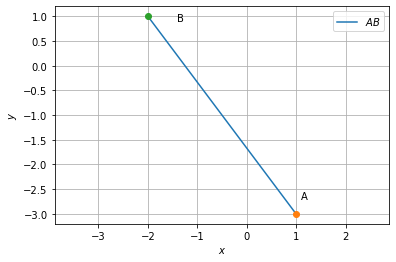
\includegraphics[width=\columnwidth]{solutions/1/8/diagram.png}
\caption{}
\label{1/8/fig:Line between A and B}
\end{figure}
